% ============================================================
% Chapter 3 -- Literature review
% ============================================================

\rev{
\chapter{Literature Review: Adaptation Under Novelty}
\label{ch:related_work}

This chapter situates the dissertation within the computational literature on learning and acting under change.
Open-set recognition, concept drift, non-stationary learning, continual learning, transfer, meta-learning, robustness, online adaptation, planning, and foundation-model agents all address some departure from training conditions or prior knowledge.
They should not, however, be collapsed into a single formulation.
They differ in what is allowed to change, what the agent is assumed to know, and what constitutes a successful response.

The conceptual perspective developed in the previous chapter provides a basis for making these distinctions.
The review asks four questions of each literature: what aspect of the environment, task, or data-generating process changes; which features, labels, states, actions, models, or task families remain fixed; what observations, feedback, and interaction are available after the change; and whether success means detection, prediction, retention, rapid adaptation, continued task performance, or revision of the agent's representation.
These questions locate the open-world problem without denying the substantial capabilities developed in neighboring areas.

The chapter first examines methods that detect unfamiliar inputs or adapt within a fixed representation, including novelty and out-of-distribution detection, concept drift, non-stationary and continual learning, transfer and meta-learning, domain randomization, and plan repair.
It then considers approaches that can extend models or behavioral structure, including open-world architectures, creative problem solving, action-model learning, and neurosymbolic systems.
Foundation models receive separate treatment because broad pretrained knowledge changes how much can be handled without task-specific learning while leaving questions of grounding, verification, and post-deployment revision unresolved.
The final synthesis uses this landscape to position the dissertation's contributions to evaluation, localized adaptation after failure, and generalization through structured abstractions.

% ============================================================
% §2.4  Existing approaches: fixed representations and representational change
% ============================================================

\section{Related Work in Learning and Planning Under Novelty}
\label{sec:what_field_does}
\label{sec:capabilities_and_gaps}

Measured against the requirements identified in \cref{sec:what_is_required}, existing methods fall into a useful pattern.
The most mature approaches support detection, re-estimation, robustness, replanning, or rapid adaptation, but often do so while keeping the agent's representational vocabulary fixed.
A smaller body of work extends the agent's representation in response to failure, but usually pays for that capacity in speed, scope, or reliance on strong structure supplied in advance.
This section organizes existing work around that trade-off.
\Cref{fig:requirements_coverage} previews the resulting picture: each method family is measured against the four requirements from \cref{sec:what_is_required}, and the survey below follows the same organization.

% Requirements coverage matrix
\begin{figure}[t]
    \centering
    \resizebox{0.98\textwidth}{!}{%
    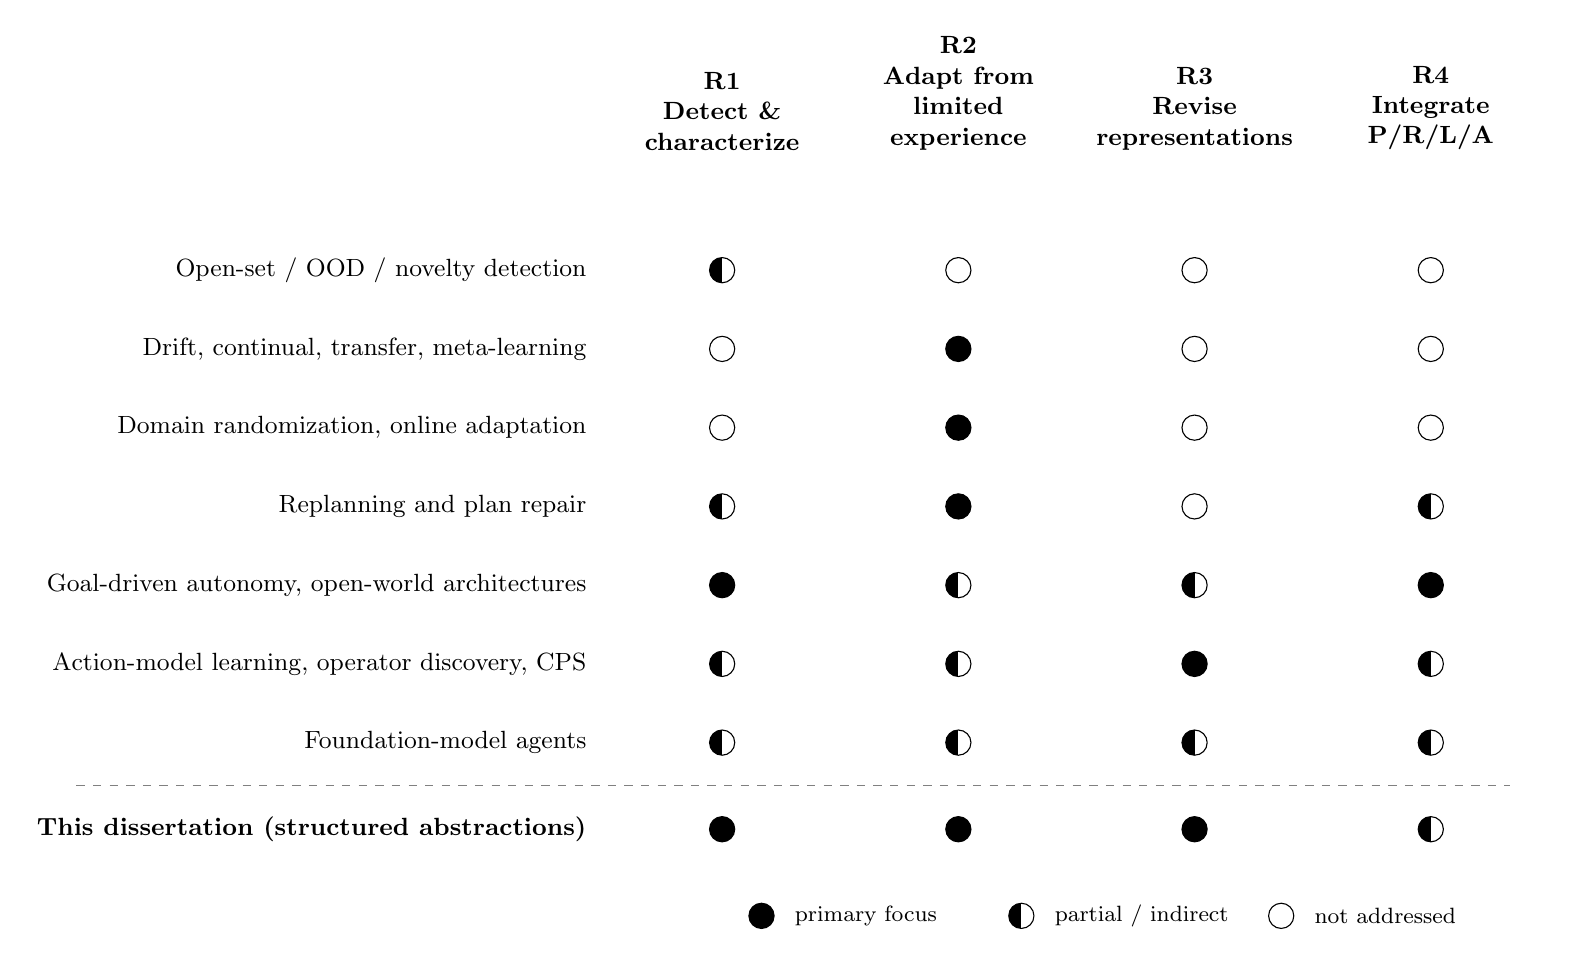
\begin{tikzpicture}[
        rowlabel/.style={anchor=east, align=right, font=\small},
        collabel/.style={anchor=south, align=center, font=\small\bfseries, text width=2.6cm},
        full/.style={circle, draw, fill=black, minimum size=0.32cm, inner sep=0pt},
        half/.style={circle, draw, minimum size=0.32cm, inner sep=0pt, path picture={\fill (path picture bounding box.south west) rectangle (path picture bounding box.north);}},
        none/.style={circle, draw, minimum size=0.32cm, inner sep=0pt},
    ]
    % Column x-positions
    \def\cA{0.0}  % R1 detect & characterize
    \def\cB{3.0}  % R2 adapt from limited experience
    \def\cC{6.0}  % R3 revise representations
    \def\cD{9.0}  % R4 integrate P/R/L/A

    % ===== Column headers =====
    \node[collabel] at (\cA, 0.4) {R1\\ Detect \&\\ characterize};
    \node[collabel] at (\cB, 0.4) {R2\\ Adapt from\\ limited experience};
    \node[collabel] at (\cC, 0.4) {R3\\ Revise\\ representations};
    \node[collabel] at (\cD, 0.4) {R4\\ Integrate\\ P/R/L/A};

    % ===== Rows =====
    % Row 1: Open-set / OOD detection
    \node[rowlabel] at (-1.6, -1.0) {Open-set / OOD / novelty detection};
    \node[half] at (\cA, -1.0) {}; \node[none] at (\cB, -1.0) {}; \node[none] at (\cC, -1.0) {}; \node[none] at (\cD, -1.0) {};

    % Row 2: Re-estimation
    \node[rowlabel] at (-1.6, -2.0) {Drift, continual, transfer, meta-learning};
    \node[none] at (\cA, -2.0) {}; \node[full] at (\cB, -2.0) {}; \node[none] at (\cC, -2.0) {}; \node[none] at (\cD, -2.0) {};

    % Row 3: Robustness / online adaptation
    \node[rowlabel] at (-1.6, -3.0) {Domain randomization, online adaptation};
    \node[none] at (\cA, -3.0) {}; \node[full] at (\cB, -3.0) {}; \node[none] at (\cC, -3.0) {}; \node[none] at (\cD, -3.0) {};

    % Row 4: Replanning / plan repair
    \node[rowlabel] at (-1.6, -4.0) {Replanning and plan repair};
    \node[half] at (\cA, -4.0) {}; \node[full] at (\cB, -4.0) {}; \node[none] at (\cC, -4.0) {}; \node[half] at (\cD, -4.0) {};

    % Row 5: GDA / open-world architectures
    \node[rowlabel] at (-1.6, -5.0) {Goal-driven autonomy, open-world architectures};
    \node[full] at (\cA, -5.0) {}; \node[half] at (\cB, -5.0) {}; \node[half] at (\cC, -5.0) {}; \node[full] at (\cD, -5.0) {};

    % Row 6: Representational extension
    \node[rowlabel] at (-1.6, -6.0) {Action-model learning, operator discovery, CPS};
    \node[half] at (\cA, -6.0) {}; \node[half] at (\cB, -6.0) {}; \node[full] at (\cC, -6.0) {}; \node[half] at (\cD, -6.0) {};

    % Row 7: Foundation-model agents
    \node[rowlabel] at (-1.6, -7.0) {Foundation-model agents};
    \node[half] at (\cA, -7.0) {}; \node[half] at (\cB, -7.0) {}; \node[half] at (\cC, -7.0) {}; \node[half] at (\cD, -7.0) {};

    % Row 8: This dissertation
    \node[rowlabel, font=\small\bfseries] at (-1.6, -8.1) {This dissertation (structured abstractions)};
    \node[full] at (\cA, -8.1) {}; \node[full] at (\cB, -8.1) {}; \node[full] at (\cC, -8.1) {}; \node[half] at (\cD, -8.1) {};

    % Separator above dissertation row
    \draw[gray, dashed] (-8.2, -7.55) -- (10.0, -7.55);

    % ===== Legend =====
    \node[full] at (0.5, -9.2) {};  \node[anchor=west, font=\footnotesize] at (0.8, -9.2) {primary focus};
    \node[half] at (3.8, -9.2) {};  \node[anchor=west, font=\footnotesize] at (4.1, -9.2) {partial / indirect};
    \node[none] at (7.1, -9.2) {};  \node[anchor=west, font=\footnotesize] at (7.4, -9.2) {not addressed};

    \end{tikzpicture}%
    }
    \caption[Method families measured against the requirements for open-world autonomy]{Method families surveyed in this chapter, measured against the four requirements for open-world autonomy identified in \cref{sec:what_is_required}: detecting and characterizing mismatch (R1), adapting from limited experience (R2), revising representations when needed (R3), and integrating perception, reasoning, learning, and action (R4). The assignments reflect the typical emphasis of each family as discussed in the text, not the capabilities of every individual system. The most mature families adapt within fixed representations (R2), while approaches that address representational revision (R3) tend to trade away speed, scope, or generality. This dissertation targets structural adaptation that is fast and localized, using structured abstractions.}
    \label{fig:requirements_coverage}
\end{figure}


\subsection{Fixed-Representation Adaptation}
\label{sec:fixed_representation_methods}

Detection methods address the first step of the open-world lifecycle (Requirement 1).
Open-set recognition formalized the problem of classification when test inputs may belong to classes absent from training, framing recognition as managing the risk of the unknown rather than discriminating among a closed label set~\citep{scheirer2013toward}.
Later work brought this capability to deep networks: OpenMax calibrates a network's activation patterns so that inputs far from all known classes can be rejected~\citep{bendale2016towards}, and \citet{hendrycks2017baseline} showed that even the maximum softmax probability provides a usable baseline signal for detecting misclassified and out-of-distribution examples.
These threads---anomaly detection, novelty detection, open-set recognition, and out-of-distribution detection---developed largely in isolation, and \citet{yang2024generalized} unify them under a single generalized framework, which is a useful map of the perceptual side of Requirement 1.
Open-world recognition extends the setting further by requiring that rejected unknowns eventually be incorporated as new classes~\citep{boult2021towards}.
This body of work is necessary for open-world autonomy, but it is not sufficient.
A classifier that rejects an unknown object, or an execution monitor that flags an unexpected outcome, has identified a mismatch.
It has not characterized the mismatch in a form that tells the agent how to recover, and it has not repaired behavior.

A related but distinct use of novelty appears in reinforcement learning as an exploration signal.
Curiosity-driven methods reward the agent for visiting states its predictive model handles poorly: the intrinsic curiosity module derives a reward from prediction error in a learned feature space~\citep{pathak2017curiosity}, and random network distillation derives one from the error of predicting the output of a fixed, randomly initialized target network~\citep{burda2019exploration}.
These methods use novelty the agent \emph{seeks} to drive exploration within a fixed observation and action space.
The setting of this dissertation is the complement: novelty is \emph{imposed} by the environment, and the question is not how to find unfamiliar states but how to recover competence when familiar ones stop behaving as modeled.
Intrinsic novelty signals can nevertheless serve Requirement 1, since the same prediction-error machinery that drives exploration can flag where an agent's model has been invalidated.

Re-estimation methods address a different part of the problem (Requirement 2).
Concept-drift methods, continual learning, transfer learning, and meta-learning can update a model as data or tasks change~\citep{gama2014survey,parisi2019continual,taylor2009transfer,finn2017maml,khetarpal2022continual}.
These methods can be powerful when the agent's representation remains adequate and only its parameters, beliefs, or policy need revision.
Their limitation is that competence is usually defined over a fixed feature, label, state, or action space.
Under structural novelty, the issue is not only that an existing probability is wrong.
The agent may lack a category, relation, precondition, or behavior needed to express the new situation.

Robotics often uses a related strategy: absorb anticipated variation before deployment.
Domain randomization trains across many simulated appearances or dynamics so that real-world variation falls inside the training envelope~\citep{tobin2017domain,peng2018sim}.
This can be highly effective for quantitative variation such as lighting, texture, mass, or friction.
Rapid motor adaptation extends the idea to online operation: a base policy is paired with an adaptation module that estimates a latent description of the current environment from recent state--action history, allowing a legged robot trained entirely in simulation to adjust to changing terrain and payloads in fractions of a second~\citep{kumar2021rma}.
This line of work shows how far Requirement 2 can be pushed when the space of variation is parameterized in advance.
It is still an assimilation strategy.
It makes more of the world look familiar, but it does not by itself introduce representational structure the designer did not anticipate.

Replanning and plan repair exploit explicit structure more directly.
When execution fails, a planner can search for a different sequence of known operators~\citep{fox2006plan,fritz2007monitoring}.
This is powerful when the current operator set contains an alternative path.
A blocked route can be bypassed; an unavailable object can sometimes be substituted.
But replanning cannot use an operator the agent does not have.
If novelty invalidates the action model itself, the agent needs more than a new plan over the same vocabulary.

\subsection{Representational Extension}
\label{sec:extend_representation_methods}

Several lines of work confront representational extension more directly (Requirement 3), often while also integrating perception, reasoning, learning, and action (Requirement 4).
An early precursor is goal-driven autonomy, in which an executing agent monitors for discrepancies between expectations and observations, generates explanations for them, and manages its own goals in response; the ARTUE agent demonstrated this detect--explain--respond loop in a Navy strategy simulation with hierarchical task network planning~\citep{molineaux2010gda}.
Goal-driven autonomy anticipated the structure of the SAIL-ON detect--characterize--accommodate framing, although its responses operate primarily at the level of goals rather than the representational vocabulary itself.
More recent open-world architectures revise the model directly: HYDRA uses model-based diagnosis over a symbolic planning model to localize which parts of the model a novelty has invalidated and to repair them, providing a domain-independent architecture for adaptive operation in evolving open worlds~\citep{mohan2024domain}.
Integrated neurosymbolic architectures similarly combine monitoring, diagnosis, symbolic reasoning, and learning to detect and accommodate novelty~\citep{muhammad2021novelty,goel2024neurosymbolic}.

A complementary line of work asks where symbolic vocabularies come from in the first place.
Action-model learning induces planning operators from experience: ARMS learns STRIPS-style action models from example plans by compiling constraints into a weighted MAX-SAT problem~\citep{yang2007arms}, LOCM induces domain models from action traces alone, without access to intermediate states~\citep{cresswell2013locm}, and later work learns action models under minimal observability by compiling the learning problem itself into classical planning~\citep{aineto2019learning}.
At the interface between control and symbols, \citet{konidaris2018skills} show that symbols representing the preconditions and effects of an agent's skills are both necessary and sufficient for high-level planning, which in principle lets an agent construct its own symbolic representation rather than receiving one from a designer.
This result matters for open-world autonomy because it implies the symbolic layer is not fixed in principle: if operators and their symbols can be learned, they can also be re-learned when the world invalidates them.
The options framework provides the underlying formalism for such temporally extended, learnable units of behavior~\citep{sutton1999options}.
SPOTTER couples symbolic planning with reinforcement learning so that an agent can learn a new operator when planning reaches an impasse~\citep{sarathy2021spotter}.
Creative problem-solving systems similarly treat execution failure as evidence that the current action model is incomplete and must be revised~\citep{gizzi2019creative,gizzi2022cps}.
These systems establish the capability this dissertation builds on: an agent can respond to failure by extending its competence rather than only by reordering known behavior.

The limitation is that representation growth is often expensive or broad.
DREAM makes representational redescription explicit, but as a developmental process operating on a slower timescale than ordinary policy learning~\citep{doncieux2020dream}.
WorldCloner shows the opposite trade-off: it adapts quickly to injected novelty by using a learned symbolic transition model, but the observation and action vocabularies remain fixed~\citep{balloch2023neuro}.
In one direction, agents can grow structure but slowly and globally; in the other, they can adapt quickly but mainly within a fixed structure.
The recurring pattern is therefore a trade-off rather than a settled solution.

This dissertation targets the space between those poles: structural adaptation that is fast and localized to the point where the world has invalidated the agent's model.
The motivating case in later chapters is an execution failure at a specific operator.
If a symbolic plan fails at \texttt{break\_tree}, the failure can identify the behavior that must be repaired.
The agent need not relearn the whole task; it can focus learning on the executor or model component whose expected effect no longer holds.
Structure matters here because it can localize the failure.

\subsection{Evaluation Gaps and Dissertation Scope}
\label{sec:ow_gaps}

Three gaps follow from this diagnosis.
First, the field needs systematic evaluation of structural novelty in sequential decision-making.
Existing SAIL-ON-inspired environments and open-world benchmarks have made novelty injection measurable~\citep{senator2019science,holder2025introduction,balloch2022novgrid,goss2023polycraft,feeney2022novelcraft}.
What remains important is evaluation that isolates how structural novelty affects performance over time: how sharply performance degrades, how quickly it recovers, and whether recovery reflects adaptation rather than accidental robustness.
\Cref{ch:benchmarks} contributes test beds and metrics for this purpose.

Second, the field needs mechanisms for failure localization and targeted skill acquisition.
Replanning can rearrange known operators, and undirected exploration can discover behavior in principle, but neither by itself identifies the exact missing competence after an execution failure.
\Cref{ch:rapid_learn} uses the structure of a failed plan to localize the problem and instantiate a focused learning task.

Third, the field needs representations that reduce unnecessary novelty by generalizing across object and embodiment variation.
Some changes look novel only because the agent's representation is too tightly tied to a particular object, robot, or control space.
\Cref{ch:flex,ch:pho} study interaction abstractions that make such variation fall within existing competence rather than requiring full retraining.

These gaps also mark the dissertation's boundaries.
The thesis does not solve open-world perception; it assumes access to task-relevant state in the main technical contributions.
It does not address safety-critical continual adaptation, where constraint violations during learning may be unacceptable~\citep{coursey2026safe}.
It also does not address the normative conflicts that arise when agents act among people and must resolve novel clashes among goals, rules, and constraints~\citep{jones2026oamncc}.
Nor does it treat novelty primarily as opportunity rather than obstacle; the methods here are failure-driven.
Those are genuine parts of open-world autonomy.
The slice addressed here is narrower: how structured abstractions support adaptation and generalization when the agent's existing model is no longer enough. However, this presents an opportunity to explore the field in a more focused way, and to develop methods that can be combined with other approaches to address the broader problem.


% ============================================================
% §3.2  Foundation models
% ============================================================

\section{Foundation Models for Open-World Autonomy}
\label{sec:foundation_models}

Foundation models, including large language models, vision--language models, and vision--language--action models, have become increasingly prominent in embodied artificial intelligence.
Their broad pretrained knowledge may help agents interpret unfamiliar situations, generate candidate plans or representations, and reduce the task-specific experience required for adaptation.
This section examines the extent to which current foundation-model systems address the requirements for open-world autonomy developed in Chapter~\ref{ch:novelty_open_world}.

% In particular, it considers what knowledge these models provide, which elements of the agent architecture and action interface remain fixed, how model outputs are grounded and verified, and whether the systems can revise their knowledge and behavior after encountering task-relevant novelty.

Recent robotics surveys document their use in perception, planning, control, simulation, human--robot interaction, and open-world execution, while also emphasizing persistent challenges in grounding, real-time control, safety, resilience, and deployment cost~\citep{khan2025foundation,sapkota2025vla}.
Foundation models can provide object knowledge, task conventions, commonsense associations, and candidate plans that may be unavailable to a narrowly trained task-specific agent.
They may therefore reduce the amount of task-specific experience required to interpret and respond to an unfamiliar situation.

The more difficult question is whether broad priors are sufficient for open-world novelty handling.
Broad prior knowledge alone does not satisfy all the requirements of open-world autonomy.
The longstanding symbol-grounding problem shifts attention from linguistic or symbolic fluency to the basis of meaning in perception and experience~\citep{harnad1990symbol,bisk2020experience}.
For an embodied agent, the operational usefulness of a concept depends on its connection to observation, action, and the consequences of acting in the environment.
NeuroAI~\citep{zador2025neuroai} arguments make the limitation more architectural than merely semantic.
Many current foundation-model systems are trained primarily from static datasets, provide limited mechanisms for continual learning after deployment, interact only indirectly with the physical world, and do not yet combine action-conditioned prediction, multi-timescale learning, and layered control in the way robust embodied agents require~\citep{zador2025neuroai}.
Cognitive-systems analyses of out-of-design-scope events make the same point in open-world terms: broad prior knowledge, fixed fallback responses, slow deliberation, and novelty-type lookup are each partial strategies, but none by itself satisfies the requirements for recognizing, characterizing, responding to, and improving from unfamiliar situations~\citep{wray2025requirements}.
% For open-world autonomy, the central issue is therefore not whether foundation models contain useful knowledge, but whether that knowledge can be made diagnosable, revisable, and grounded in action.

% Early language-model agents for embodied tasks illustrate both the promise and the boundary.
Language models can decompose high-level instructions into plausible action sequences, especially when their outputs are mapped onto admissible actions~\citep{huang2022language}.
SayCan adds an important grounding step by combining language-model scores with value functions over available robot skills, so that task knowledge is constrained by what the robot can actually do~\citep{ahn2022can}.
Vision--language--action models such as RT-2 go further by transferring web-scale vision-language knowledge into robotic control, improving generalization to novel objects and instructions~\citep{pmlr-v229-zitkovich23a}.
These systems contribute to aspects of the first, second, and fourth requirements: they broaden perceptual and semantic interpretation, make action selection more flexible, and may reduce the amount of task-specific experience required.
However, many models still require task- and embodiment-specific fine-tuning~\citep{ma2026survey}.
Their principal limitation in this setting is that they largely operate over a fixed action interface, a learned policy, or a predefined set of skills.
When novelty invalidates the agent's model, the system still needs a way to identify what failed, decide whether the failure is perceptual, symbolic, or motoric, and revise the relevant representation.

Planning provides a concrete setting in which the reliability of model-generated structure can be evaluated against explicit states, actions, and goal conditions.
\citet{valmeekam2023planning} evaluate large language models on plan generation in domains modeled on International Planning Competition benchmarks and find that autonomous plan generation is weak---the best model in their study, GPT-4, solves roughly 12\% of instances on average---while the models are more useful as a source of heuristic guidance for external planners.
In a recent Blocksworld study, \citet{gobel2026agentic} report a similar pattern when comparing direct language-model planning and stepwise PDDL-simulation-guided language-model planning against a classical planner.
The classical planner solves a larger fraction of instances, while the language-model variants remain substantially weaker and the agentic version yields only modest gains at much higher token cost.
These results should not be read as a dismissal of language models.
They support a narrower but important point: broad linguistic priors do not replace compositional search, explicit state update, and externally checkable plan structure when reliability matters.
The literature on creative problem solving raises a related concern.
\citet{nair2024cps} argue that large language and vision models still struggle to generate genuinely new concepts when existing ones are insufficient.
In the terminology of this chapter, that is an accommodation problem: the agent must form and test a new representational commitment, not merely produce a fluent continuation of an old one.

Open-ended language-model agents show a different kind of strength.
MineDojo established the infrastructure for this line of work, pairing a Minecraft-based benchmark of thousands of open-ended tasks with an internet-scale knowledge base of videos, wiki pages, and forum discussions from which agents can draw priors~\citep{fan2022minedojo}.
Voyager uses a language model to propose goals and write executable code in Minecraft, accumulating a skill library that transfers across worlds~\citep{wang2023voyager}.
DECKARD makes the proposal-verification structure explicit: a language model hypothesizes an abstract world model of subgoals and their dependencies, and the agent verifies or corrects the hypothesized model against grounded experience, improving sample efficiency by an order of magnitude while remaining robust to errors in the language model's knowledge~\citep{nottingham2023deckard}.
Odyssey similarly develops Minecraft agents around open-world skill libraries and benchmarks for long-horizon planning, dynamic planning, and autonomous exploration~\citep{liu2025odyssey}.
These systems are important demonstrations of repertoire expansion.
They also clarify the boundary between open-ended exploration and open-world recovery.
They expand an agent's behavioral repertoire inside rich but comparatively well-specified interfaces; they do not fully address the case in which an ongoing task fails because the agent's model of objects, operators, constraints, or executors has become wrong and must be repaired.

The work closest to the requirements treats foundation models as components in structured adaptation loops.
\citet{kumar2026openworldtamp} use vision-language models to generate constraints for open-world task and motion planning, allowing a planner to reason about goals and scene properties not fully specified in the original domain model.
\citet{yang2025skillwrapper} use foundation models for predicate invention, learning human-interpretable symbolic predicates that wrap black-box robot skills into operators suitable for planning.
\citet{li2026recover} learn recovery skills from robot failures and discover relational concepts that let local recoveries become reusable planning knowledge.
\citet{lu2026novelty} use a language model to identify missing operators after novelty, a symbolic planner to incorporate them, and language-model-written rewards to guide reinforcement learning for the corresponding control policies.
\citet{lorang2025fewshot} similarly combine symbolic abstraction with continuous controllers learned from few demonstrations.
Across these systems, the foundation model is most useful when it proposes candidate constraints, predicates, operators, rewards, or skills into an architecture that can localize failure, test the proposal, and connect it to action.

Foundation models widen the priors available to an agent and can support multiple forms of generalization.
They do not, by themselves, remove the need for open-world mechanisms of characterization, representation revision, verification, and grounded learning.
Taken together, the reviewed studies suggest an architectural role for foundation models as sources of candidate knowledge and structure.
Foundation models can propose constraints, predicates, operators, rewards, plans, or skills, while complementary mechanisms localize mismatch, test the proposals, ground them through interaction, and revise the agent's knowledge when necessary.
On this account, model-based proposal and structured verification provide complementary capabilities for open-world autonomy.


% ============================================================
% §3.3  Synthesis and positioning
% ============================================================

\section{Synthesis: Open-World Autonomy and Dissertation Scope}
\label{sec:synthesis_positioning}
\label{sec:ow_gaps}
\label{sec:positioning}
\label{sec:open_world_landscape}
\label{sec:related_work_positioning}
\label{sec:perspectives_integration}
\label{sec:ch3_positioning_summary}

The literature shows that open-world autonomy is not synonymous with learning from non-identically distributed data or adapting after a task change.
Open-set and out-of-distribution methods emphasize detection relative to a reference distribution.
Concept-drift and non-stationary methods track changes in distributions, rewards, or dynamics.
Continual learning emphasizes accumulation and retention across experience, transfer learning exploits relations between source and target problems, and meta-learning acquires procedures for rapid adaptation across a task distribution.
Domain randomization and online adaptation enlarge the range of anticipated variation that an existing policy can tolerate, while replanning searches for an alternative sequence of known actions.
Each of these capabilities is relevant to an open-world agent, but none alone addresses the full case in which the assumptions or representation supporting the agent's behavior become inadequate.

This comparison reveals two broad regimes rather than a categorical separation among research communities.
When the relevant classes, variables, actions, and dimensions of variation have been anticipated, an agent can respond by updating beliefs, parameters, or policies within an adequate representation.
When they have not, continued action may require the agent to learn or revise a concept, relation, operator, transition model, skill, or goal.
Methods that support such revision confront a broader class of change, but they also expose a recurring trade-off: representational extension is often slower, more global, or more dependent on structure supplied in advance.

Foundation models change the scale of prior knowledge available to an agent but not this underlying problem.
Their broad semantic and behavioral priors can make additional situations assimilable without task-specific learning, and they can propose candidate structure when existing knowledge is insufficient.
Yet a situated agent still requires mechanisms for determining what failed, deciding what kind of revision is needed, testing candidate revisions, and grounding them in the consequences of action.
The gap is therefore not simply a lack of prior knowledge; it is the lack of reliable mechanisms that connect experienced mismatch to an appropriately scoped representational response.

The distinction between assimilation and accommodation provides a compact interpretation of this boundary without replacing the more specific problem definitions above.
Structured abstractions mediate both responses to novelty.
By encoding task-relevant invariances, they can expand the range of environmental variation that an agent assimilates within its existing knowledge and behavior.
By decomposing knowledge and behavior into identifiable, revisable components, they can make accommodation localizable when that knowledge or behavior is no longer sufficient.
A monolithic policy may register novelty only as degraded performance, whereas a structured agent can sometimes identify the failed operator, executor, object relation, or interaction variable and restrict revision to the component that no longer matches the world.

In this dissertation, we address a specific subset of the broader open-world problem through three complementary contributions.
First, systematic progress requires environments in which diverse agents can be developed and compared under controlled change.
Existing SAIL-ON-inspired environments and open-world benchmarks have made novelty injection measurable~\citep{senator2019science,holder2025introduction,balloch2022novgrid,goss2023polycraft,feeney2022novelcraft}.
In \cref{ch:benchmarks}, we present \NovelGridworlds{} and \NovelGym{}, configurable environments that support modular transformations of entities, actions, tasks, and dynamics, together with protocols and metrics for characterizing the impact of novelty and the subsequent course of adaptation.
The accompanying software ecosystem supports the development and evaluation of modular agent architectures designed for open-world settings.
This contribution operationalizes the study of how novelty affects existing knowledge and behavior and when an adaptive response becomes necessary.

Second, open-world agents require mechanisms for localized accommodation after execution failure.
Replanning can rearrange known operators, and undirected exploration can discover behavior in principle, but neither by itself identifies the precise missing behavior when an expected action effect no longer occurs.
In \cref{ch:rapid_learn}, we study action abstractions in which symbolic operators are associated with executable behaviors.
When an executor fails, the intended effects of its operator define what recovery must accomplish, converting global task failure into a targeted skill-learning problem while preserving unaffected knowledge and behaviors.

Third, agents should not be forced to accommodate every change they encounter.
Some apparent novelty results from representations that are unnecessarily tied to a particular object, physical condition, robot, or control space.
In \cref{ch:flex,ch:pho}, we study interaction abstractions that represent manipulation at the level of object interaction rather than robot-specific control.
By capturing forces, object dynamics, and other task-relevant invariances, these abstractions allow existing skills to generalize across objects, physical parameters, and embodiments; in the terminology of this chapter, they expand the range of variation that can be assimilated without structural revision or retraining.

The action and interaction contributions therefore instantiate complementary consequences of the framework taken from \cref{ch:novelty_open_world}.
Action abstractions provide structured interfaces for accommodation when novelty invalidates an existing behavior.
Interaction abstractions enlarge the domain of assimilation by making some environmental and embodiment variation irrelevant to the learned skill.
The benchmark contribution makes these responses available for controlled study and evaluation.
Together, they support the thesis that representational structure shapes whether environmental change produces brittle failure, targeted accommodation, or continued task performance through generalization.

These contributions address only part of the broader problem of open-world autonomy.
They do not solve general open-world perception, autonomously construct arbitrary ontologies, or integrate all four requirements into a single lifelong agent.
The main technical contributions assume access to task-relevant state and do not address safety-critical continual adaptation, where violations during learning may be unacceptable~\citep{coursey2026safe}.
They also do not address the normative conflicts that arise when agents operating among people encounter novel clashes among goals, rules, or constraints~\citep{jones2026oamncc}.
Finally, the methods are primarily failure-driven and do not treat novelty principally as an opportunity for self-directed exploration or goal formation.
Instead, they isolate and study how explicit structure can support evaluation, localized behavioral accommodation, and generalization across important classes of variation.
These boundaries define the scope of the dissertation rather than the scope of open-world autonomy as a whole.
The next chapter formalizes the agent--environment setting, the notion of novelty, and the action and interaction abstractions used to develop these claims in the technical chapters.

}
